\chapter{Expectation Maximization}
\label{ch:em}

\textbf{Expectation maximization} is a method that allows us to perform \textit{maximum likelihood} inference in scenarios where computing the likelihood explicitly may not be possible because of the presence of \textbf{latent variables}.

\subsection*{Learning Bayesian Networks}

We will start by focusing on a simpler problem to set the scene. Remember that a BN is a way to factorize a joint distribution according to:

$$
p(x) = \prod_{i}p(x_i|pa(x_i))
$$

We know how to compute inference, marginals, etc... but how can we learn Bayesian Networks from data? Here we focus on the problem of learn parametric models of conditional distributions, for a fixed structure of the BN.

We typically have that each factor $p(x_i|pa(x_i), \theta_i)$ depends also on some parameters $\theta_i$ which can be estimated by Maximum likelihood (ML) from data. 

Let's start with the following example
\vspace{0.5cm}
\begin{center}
    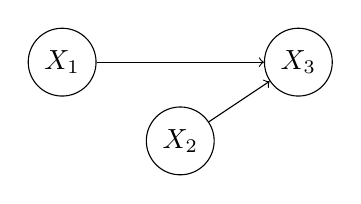
\begin{tikzpicture}
        % Nodes 
        \node(x1) [circle, draw] at (-1.5,0) {$X_1$};
        \node(x2) [circle, draw] at (0,-1) {$X_2$};
        \node(x3) [circle, draw] at (1.5,0) {$X_3$};
        
        % Edges
        \draw[->] (x1) -- (x3);
        \draw[->] (x2) -- (x3);
    
    \end{tikzpicture}
\end{center}

$$
p(X_1, X_2, X_3) = p(X_3|X_1, X_2)p(X_1)p(X_2)
$$

and suppose that $x_i \in \{0,1\}$. Focus on learning the factor $p(x_3|x_1,x_2)$ and consider all the possible value in the conditioning set. Therefore we want to learn the following values:

$$
\begin{array}{c}
    p(x_3 = 1|x_1 = 0, x_2 = 0) = \theta_{00} \\
    p(x_3 = 1|x_1 = 0, x_2 = 1) = \theta_{01} \\
    p(x_3 = 1|x_1 = 1, x_2 = 0) = \theta_{10} \\
    p(x_3 = 1|x_1 = 1, x_2 = 1) = \theta_{11} \\
\end{array}
$$

Learning by maximum likelihood these parameters just means computing 

$$
\theta_{ij} = \frac{\#(x_1 = i, x_2 = j, x_3 = 1)}{\#(x_1 = i, x_2 = j)},
$$

where the notation $\#$ returns the cardinality of the set of observations satisfying the constraint in brackets. 

\textbf{Remark.} In a continuous setting you may want to model $p(x_3|x_1,x_2)$ as a combination of values of $x_1, x_2$. The specific choice of the parametric model depends on what is the phenomena you are trying to model.

In this context, as long as the number of parents of each $x_i$ is relatively small, computations are feasible. What happens though if we don't observe, for example, $x_1$? We cannot employ this model for latent variables!

\subsection*{Problem formulation}

Let's consider a more general scheme like the following: we have a certain number of variables $x$ which are observed and a set of variables $z$ which is unobserved. Generally speaking, we will have a parametric model $p(x,z|\theta)$ and we would like to compute $\theta_{ML}$. In order to identify $\theta_{ML}$ we need to optimize the marginalized likelihood on $x$:

$$
p(x|\theta) = \sum_z p(x,z|\theta)
$$

If $z$ is high-dimensional, we would to sum over exponentially many possible states, which makes our problem intractable. 

The problem becomes even more complex when we have $\underbar{x} = x_1, \dots, x_n$ observations and $\underbar{z} = z_1, \dots, z_n$ latent states of observations since we would like to work with the logarithm of our distribution for numerical stability 

$$
p(\underbar{x}, \underbar{z}|\theta) = \prod_n p(x_n, z_n|\theta) \quad \log p(\underbar{x}, \underbar{z}|\theta) = \sum_n \log p(x_n, z_n|\theta) 
$$

but then 

$$
\log p(\underbar{x}|\theta) \neq \sum_n \log p(x_n|\theta) 
$$

because of the summation over $z$ in the definition of $p(x|\theta)$.

\section{Evidence lower bound}

Again, consider a joint model $p(x,z)$ with $x$ observed and $z$ unobserved with corresponding observations $x_1, \dots, x_n$ and latent states $z_1, \dots, z_n$. Our goal is to compute $p(x|\theta) = \sum_n p(x,z|\theta)$ and we want to learn $\theta_{ML}$, i.e. $\theta$ such that 

$$
\argmax{\theta} p(\underbar{x}|\theta) 
$$

This problem is typically intractable for the reasons described before.

We still introduce a key approximation which will also be useful for variational inference. Consider 

$$
p(x,z|\theta) = p(x|\theta)p(z|x,\theta) 
$$

The idea is to approximate $p(z|x,\theta)$ with the so called \textbf{variational approximation} $q(z)$ (which can be any distribution over $z$). 

Let's consider the \textbf{Kullback-Leibler divergence} of $q$ and $p$ 

$$
KL[q||p] = KL[q(z)||p(z|x,\theta)] = \mathbb{E}_{q(z)}\left[-\log \frac{p(z|x,\theta)}{q(z)}\right] = -\sum_z q(z)\log \frac{p(z|x,\theta)}{q(z)}
$$

The trick now is to add and subtract the term $|\log p(x|\theta)$ in the logarithm 

$$
-\sum_z q(z)\log\frac{p(z|x,\theta)}{q(z)} = -\sum_z q(z)\left[\log\frac{p(z|x,\theta)}{q(z)} + \log p(x|\theta) - \log p(x|\theta)\right] 
$$

And then we can start to aggregate these factors obtaining

$$
KL[q(z)||p(z|x,\theta)] = -\underbrace{\sum_z q(z)\log\frac{p(x,z|\theta)}{q(z)}}_{\text{ELBO}} + \log p(x|\theta)
$$

\begin{definitionblock}[ELBO]
    $$
    \mathcal{L}(q, \theta) = \sum_z q(z)\log\frac{p(x,z|\theta)}{q(z)}
    $$

    is the \textbf{Evidence Lower Bound} (also called \textbf{ELBO}).
\end{definitionblock}

From the expression above we can rewrite our log likelihood as 

$$
\log p(x|\theta) = \mathcal{L}(q,\theta) + KL[q(z)||p(z|x,\theta)]
$$

\textbf{Remark.} Since $KL[q|p] \geq 0$ then $\mathcal{L}(q,\theta) \leq \log(p(x|\theta))$ i.e. it is a lower bound for the log likelihood.

Whenever we have a tractable form for $p(x,z|\theta)$ then the ELBO is also tractable. Expectation Maximization will actually optimize the ELBO with respect to both $\theta$ and $q$ (since $q$ is a distribution we are using the tools of variational calculus to perform this optimization) in an "alternated" fashion (optimize with respect to one and the other argument in two different steps).

\section{Expectation Maximization}

Let's start from this expression for the ELBO 

$$
\mathcal{L}(q,\theta) = \mathbb{E}_q\left[\log\frac{p(x,z|\theta)}{q(z)}\right] = \underbrace{\mathbb{E}_q[\log p(x,z|\theta)]}_{\text{Energy term}} + \underbrace{\mathbb{E}_q[-\log q(z)]}_{\text{Entropy} (H(q))}
$$

The first term is called the \textbf{Energy term}, while the second term is actually the entropy of the $q$ distribution (written $H(q)$).

The goal of the EM algorithm is to find $\theta_{ML} = \argmax{\theta} \log p(\underbar{x}|\theta)$ which, since it is analitically intractable as we have seen, will lead us to maximize the ELBO, in both $q$ and $\theta$.

The way in which we proceed is to maximize for each variable on different steps. The maximization with respect to $q$ is known as the \textbf{expectation maximization} step (or the m-step).

\subsection*{E-step}

Let's fix $\theta$ to $\theta_{OLD}$. We need to solve an optimization problem in a function space. This is easy though if we notice that $\mathcal{L}(q,\theta)$ is maximum whenever $KL[q(z)||p(z|\underbar{x},\theta)] = 0$, since $\log p(\underbar{x}|\theta)$ does not depend on $q$ and 

$$
\mathcal{L}(q,\theta) = \log p(\underbar{x}|\theta) - KL[q(z)||p(z|\underbar{x},\theta)]
$$

Therefore 

$$
q_{max} = p(\underbar{z}|\underbar{x},\theta_{OLD})
$$

where 

$$
p(\underbar{z}|\underbar{x},\theta) = \prod_{i=1}^N p(z_i|x_i,\theta) \quad \text{if } x_1, \dots, x_n \text{ are i.i.d}
$$

Then we compute $\mathbb{E}_{q_{new}}[\log p(\underbar{x},z|\theta)]$ as a function of $\theta$ and the e-step is completed.

\textbf{Remark.} In order for the EM algorithm to work effectively, we need to be able to evaluate analytically or numerically the conditional distribution $p(\underbar{z}|\underbar{x},\theta_{OLD})$.

\subsection*{M-step}

Now we need to maximize $\mathcal{L}(q,\theta)$ keeping $q$ fixed to $q = q_{new} = p(\underbar{z}|\underbar{x},\theta_{OLD})$ which is tantamount to maximize w.r.t. $\theta$

$$
\mathbb{E}_{q_{new}}[\log p(z,\underbar{x}|\theta)]
$$

i.e. the energy term.

This maximization really depends on the problem at hand, but usually is just about explicitly computing the gradient, setting it to zero, and find 

$$
\theta_{new} = \argmax{\theta} \mathbb{E}_{q_{new}}[\log p(\underbar{x},z|\theta)]
$$

The algorithm works by repeating these two steps until convergence (i.e. whenever $||\theta_{OLD} - \theta{NEW}|| < \epsilon$). The reason why this works is easily explained in a graphical way.

\begin{figure}[H]
    \centering
    \includegraphics[width=0.4\textwidth]{assets/fig35.png}
    \label{fig:em1}
\end{figure}

After setting the Kullback-Leibler divergence to zero, we close the gap vertically and we make the log-likelihood equal to the lower bound.

\begin{figure}[H]
    \centering
    \includegraphics[width=0.4\textwidth]{assets/fig36.png}
    \label{fig:em2}
\end{figure}

In the M-step, since we are maximizing the lower bound, we are pushing it up, but then also the log-likelihood will be pushed up, possibly of a larger quantity than the lower bound, creating a new gap.

After both the E and M steps are completed, the log-likelihood is always increasing, until it gets really close to a local maximum and eventually reaches it. So we can consider as the termination condition of the EM algorithm the following: $\mathcal{L}(q_{NEW},\theta_{NEW}) - \mathcal{L}(q_{OLD},\theta_{OLD}) < \delta$, where $\delta$ is a chosen constant.

\textbf{Remark.} In general the EM algorithm converges to a \textbf{local} optimum of $\log p(\underbar{x}|\theta)$.

\textbf{Remark.} If $p(\underbar{z}|\underbar{x},\theta)$ is not easily computable, we can use a $q$ that is an approximation. In this case EM interactions will reduce $KL(q||p)$ but it will not be set to zero, hence convergence is not guaranteed.

\section{Mixture of Gaussians}

We will see an application of the EM algorithm in a typical scenario.

Let's start with a graphical representation of a Gaussian Mixture model:

\begin{figure}[H]
    \centering
    \includegraphics[width=0.15\textwidth]{assets/fig37.png}
    \label{fig:em3}
\end{figure}

where $z$ is a discrete R.V. $z_1,\dots, z_k, z_j \in \{0,1\}, \sum_j z_j = 1$ which means that we have a \textbf{one-hot-encoding} representation for $z$. $\pi$ is a discrete probability distribution that defines the probability of being assigned to the j-th component of the Gaussian mixture, while $\mu, \sigma^2$ are the mean and the variance of each Gaussian distribution.

Moreover we have N observations of $x$ which means that we also have N corresponding $z$ unobserved realizations of the variable $\underbar{z} = (z_{ij}), i = 1, \dots, N, j = 1, \dots, k$.

The joint distribution for the GMM model, using the one-hot encoding representation for our variates is 

$$
p(x,z|\theta) = \underbrace{\prod_{j=1}^K \pi_j^{z_j}}_{p(z|\theta)} \cdot \underbrace{\mathcal{N}(x|\mu_j,\sigma_j^2)^{z_j}}_{p(x|z,\theta)}
$$

where notice that $z_j$ is 1 only for one j-th component and zero otherwise, which means that in the product we only really get one factor (the others are all 1).

This is not the typical thing that we write for a mixture of Gaussians though: since we don't observe $z$, we need to write the marginal distribution 

$$
p(x|\theta) = \sum_{j=1}^K \pi_j \mathcal{N}(x|\mu_j,\sigma_j^2)
$$

The problem is that the direct optimization of this is intractable. Then we also need to consider the other terms that we need in our algorithm, i.e. 

$$
\begin{array}{c}
    p(z|\theta) = \prod_j \pi_j^{z_j} \\
    p(z|\underbar{x},\theta) \propto \prod_{n=1}^N \prod_{j=1}^K \pi_j^{z_{nj}} \mathcal{N}(x_n|\mu_j,\sigma_j^2)^{z_{nj}} \\
    p(z = j|x,\theta) = \frac{\pi_j\mathcal{N}(x|\mu_j,\sigma_j^2)}{\sum_{i=1}^K\pi_i\mathcal{N}(x|\mu_i,\sigma_i^2)}
\end{array}
$$

where the last probability distribution is considered since we have seen that, given i.i.d. r.v., our conditional distribution factorizes as $p(\underbar{z}|\underbar{x},\theta) = \prod_{i=1}^N p(z_i|x_i,\theta)$.

In this model we can easily evaluate the conditional distribution of $z$ given $x$, which is what makes the computation of the EM algorithm effective.

Then it is relatively simple to comptute

$$
\mathbb{E}_{p(z|x)}[z_{nj}] = p(z = j|x_n,\theta) = \frac{\pi_j\mathcal{N}(x_n|\mu_j,\sigma_j^2)}{\sum_i\pi_i\mathcal{N}(x_n|\mu_i,\sigma_i^2)} := \gamma(z_{nj})
$$

which is called the \textbf{responsibility} in the gaussian mixture model scenario, and it is needed to compute what we actually care about for the e-step of the EM, which is the expectation of 

$$
\log p(\underbar{x},\underbar{z}|\theta) = \sum_{n=1}^N \sum_{j=1}^K z_{nj}[\log \pi_j + \log \mathcal{N}(x_n|\mu_j,\sigma_j^2)]
$$

that is 

$$
\mathbb{E}_{p(\underbar{z}|\underbar{x},\theta)}[\log p(\underbar{x},\underbar{z}|\theta)] = \sum_{n=1}^N \sum_{j=1}^K \mathbb{E}[z_{nj}][\log \pi_j + \log \mathcal{N}(x_n|\mu_j,\sigma_j^2)]
$$

Now we can solve in close form the optimization problem, which means that we can compute analytically the derivatives with respect to our parameters in order to determine the maxima. Performing calculations we find 

$$
\begin{array}{c}
    \mu_j^{new} = \frac{1}{N_j}\sum_n \gamma(z_{nj})x_n \\
    \Sigma_j^{new} = \frac{1}{N_j}\sum_n \gamma(z_{nj})(x_n - \mu_j^{new})^T(x_n - \mu_j^{new}) \\
    \pi_j^{new} = \frac{N_j}{N}, \quad N_j = \sum_{n=1}^N \gamma(z_{nj}) \\
\end{array}
$$

where $\pi_j^{new}$ is the count of the probability that each observation comes from the j-th component over all the observations; $\mu_j^{new}$ is a weighted mean of the variables $x$ for all the observations that comes from component $j$; $\Sigma_j^{new}$ is again a weighted average of all the covariances. 

\textbf{Remark.} A good initial guess for the parameters for our algorithm is given by runing a k-means clustering and considering the averages and covariances of each cluster as a starting value for $\mu_j$ and $\Sigma_j$. In fact, k-means could be thought of as an approximation of EM, where covariances are assumed to be identical and spherical. 

\newpage 
\section{EM for Bayesian Networks}

We are going back to the motivating example that we have seen in the introduction to explain how to solve the problem we posed. 

Let's consider a BN on a certain set of variables such that their joint distribution is such that 

$$
p(x) = \prod_i p(x_i|pa(x_i),\theta_i)
$$

And also we have our usual assumption that the set of variables $x$ is divided into a set of visible (observable) variables $v$, and a set of hidden variables $z$. We can alternatively write then 

$$
p(x) = p(v,z|\theta) 
$$

In general, we need to consider how to compute 

$$
p(z|v=\hat{v},\theta)
$$

for fixed $\theta$, which we need to compute the expectation step. This conditional, in the Bayesian settings scenario, is very easily computable using belief propagation. 

Let us denote with $\underbar{v} = (v_1, \dots, v_n)$ the set of observations of $v$, then our goal is to do maximum likelihood (using the expectation maximization algorithm) to compute the best $\theta$ for our distribution. Define 

$$
q^n(z) := p(z|v_n,\theta) 
$$

which is our conditional distribution for each possible observation of $v$. We can also extend it to all variables $x$, by means of the delta distribution 

$$
q^n(x) =  p(z|v,\theta)\delta(v,v_n)
$$

The e-step then just boils down to computing this $q^n(x)$. For the m-step we need the energy 

$$
\sum_n \mathbb{E}_{q^n}[\log p(v_n,z_n|\theta)] = \sum_n \sum_i \mathbb{E}_{q^n}[\log p(x_i^n|pa(x_i^n)|\theta_i)]
$$

Then we can optimize 

$$
\sum_n \mathbb{E}_{q^n}[\log p(x_i^n|pa(x_i^n)|\theta_i)]
$$

over $\theta_i$ for each $i$.

Let's introduce an example to make it clearer. Consider this simple structure 

\vspace{0.5cm}
\begin{center}
    \begin{tikzpicture}
        % Nodes 
        \node(z) [circle, draw, minimum size=1.5cm] at (-2.5,0) {$z$};
        \node(v) [circle, draw, minimum size=1.5cm] at (2.5,0) {$v$};
        \node(w) [circle, draw, minimum size=1.5cm] at (0,-2) {$w$};

        % Edges
        \draw[->] (z) -- (w);
        \draw[->] (v) -- (w);
    \end{tikzpicture}
\end{center}

and each of the variables is boolean. The probability distributions are defined by the parameters 

$$
\begin{array}{c}
    p(z = 1) = \theta_z \\
    p(v = 1) = \theta_v \\
    p(w = 1|z = a, v = b) = \theta_{wab}, \quad a,b \in \{0,1\} \\
\end{array}
$$

Assume that we have observations $(v_1,w_1), \dots, (v_n,w_n)$. The e-step for each observation just corresponds to find the distribution 

$$
q^n(z) = p(z|v = v_n, w = w_n, \theta)
$$

or, as a function of $x$

$$
q^n(x) = p(z|v = v_n, w = w_n, \theta)\delta(v,v_n)\delta(w,w_n)
$$

Let's write the energy term for a couple of factors to get an idea of how to compute it and how to optimize with respect to it 

$$
\sum_n \mathbb{E}_{q^n}[\log p(z^n|\theta_z)] = \sum_n \log \theta_z q^n(z = 1) + \log(1 - \theta_z)q^n(z = 0)
$$

If we maximize this with the constraint $\theta_z \in [0,1]$ we obtain 

$$
\theta_z = \frac{\sum_n q^n(z=1)}{\sum_n q^n(z=1) + \sum_n q^n(z=0)} = \frac{1}{N}\sum_n q^n(z=1)
$$

A second (slighly more complicated) example is the energy term with respect to $w$, i.e. 

$$
\sum_n \mathbb{E}_{q^n}[\log p(w_n|z,v_n,\theta_w)]
$$

let's restric to the case $z = 0,  v = 1 \quad (\theta_{w01})$

$$
\sum_{n:w_n=1v_n=1} q^n(z=0)\log \theta_{w01} + \sum_{n:w_n=0,v_n=1} q^n(z=0)\log(1-\theta_{w01})
$$

Maximizing over this yields 

$$
\theta_{w01} = \frac{\sum_n \mathcal{F}(w_n = 1)\mathcal{F}(v_n = 1)q^n(z = 0)}{\Sigma_n\mathcal{F}(w_n = 1)\mathcal{F}(v_n = 1)q^n(z = 0) + \Sigma_n\mathcal{F}(w_n = 0)\mathcal{F}(v_n = 1)q^n(z = 0)}
$$

\section{EM for Hidden Markov Models}

We are going to address how to use the Expectation Maximization algorithm in the context of Hidden Markov Models, which, remember, are just a special case of Bayesian Networks. Let's consider the following HMM:

\vspace{0.5cm}
\begin{center}
    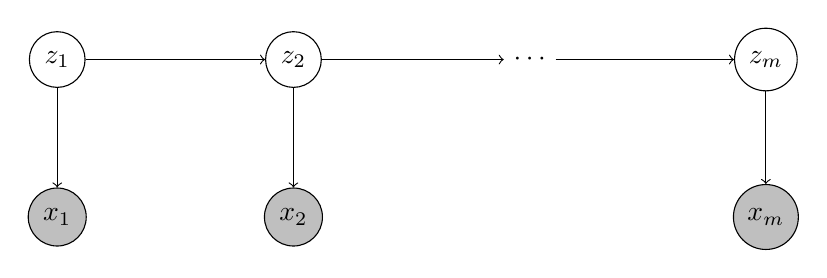
\begin{tikzpicture}
        % nodes
        \node(z1) [circle, draw] at (-6, 0) {$z_1$};
        \node(z2) [circle, draw] at (-3, 0) {$z_2$};
        \node(zm) [circle, draw] at (3, 0) {$z_m$};
        \node(x1) [circle, draw, fill=gray!50] at (-6, -2) {$x_1$};
        \node(x2) [circle, draw, fill=gray!50] at (-3, -2) {$x_2$};
        \node(xm) [circle, draw, fill=gray!50] at (3, -2) {$x_m$};

        \node(dots) at (0,0) {$\cdots$};

        %edges
        \draw[->] (z1) -- (z2);
        \draw[->] (z2) -- (dots);
        \draw[->] (dots) -- (zm);
        \draw[->] (z1) -- (x1);
        \draw[->] (z2) -- (x2);
        \draw[->] (zm) -- (xm);

    \end{tikzpicture}
\end{center}

with each $z_i \in \{1, \dots, k\}$ being a categorical variable, we have the following probability distributions 

$$
\begin{array}{c}
    p(z_1 = i) \pi_i \\
    p(z_i = j|z_{i-1} = k) = A_{kj} \\
    p(x_i|z_i = k) = p(x_i|\phi_k) \\
    \theta = (\pi, A, \phi)
\end{array}
$$

The EM algorithm for Hidden Markov model is known as the \textbf{Baum-Welch algorithm}.

The observation set in this context corresponds to whole trajectories (all the $x$ variables of the model are observed in each trajectory). We will write them as $\underbar{x} = x^1, \dots, x^N$ where each $x^i = (x_1^i, \dots, x_M^i)$.

For the e-step, we need to compute 

$$
q^n(z) = p(z|x^n, \theta_{OLD})\quad \forall n 
$$

and this is done just by running our message passing algorithm for Bayesian Networks. For the m-step instead, we want 

$$
    E(\theta) = \sum_{n=1}^N\left[\sum_{k=1}^K q^n(z_{1k})\ln\pi_k + \sum_{i=2}^M \sum_{j,k=1}^K q^n(z_{(i-1)},z_{ik})\ln A_{jk} + \sum_{i=1}^M\sum k=1^Kq^n(z_{ik})\ln p(x_i^n|\phi_k)\right] 
$$

Then we just need to maximize over all the parameters belonging to theta, i.e. $\theta = (\pi, A, \phi)$.

Working on the calculations we get, for example for $\pi_k$ 

$$
\pi_k = \frac{\Sigma_nq^n(z_{1k})}{\Sigma_i\Sigma_n q^n(z_{1i})}
$$

Similarly, we can obtain expressions for the other parameters. 
